\documentclass[conference]{IEEEtran}
\usepackage[T1]{fontenc}
\usepackage{cite,graphicx,amsmath,amssymb,booktabs,array,url,tikz,balance}
\usetikzlibrary{arrows.meta,positioning,shapes.geometric}
\graphicspath{{./}}
\title{Voice-Based Parkinson's Disease Classification Using Handcrafted Acoustic Features and Log-Mel Spectrograms}
\author{\IEEEauthorblockN{Suvinay Foujdar, Akshat Goyal, and Navya Loshali}
\IEEEauthorblockA{Department of Computer Science and Engineering\\Bennett University, Greater Noida, India}}
\begin{document}
\maketitle
\begin{abstract}
Parkinson's disease (PD) can affect speech production, motivating research into voice recordings as a non-invasive source of acoustic information. This study compares a classical machine-learning pipeline based on handcrafted acoustic summaries with a convolutional neural network (CNN) based on Log-Mel spectrograms. The experiments use an Italian Parkinson's Voice and Speech collection containing 831 WAV recordings from 65 participants: 37 healthy controls and 28 participants with PD. Participants, rather than individual recordings, are assigned to disjoint development and test partitions. Four classical classifiers are evaluated using five-fold participant-stratified cross-validation, and an RBF-kernel support vector machine (SVM) is selected. A separate CNN processes five-second, 64-band Log-Mel inputs. On 226 held-out recordings from 17 participants, the SVM achieves 0.9558 recording-level accuracy and 0.9412 participant-level accuracy; the CNN achieves 0.9690 and 0.9412, respectively. The SVM has a higher recording-level ROC-AUC, while both models have identical participant-level metrics in the saved run. The small held-out cohort and absence of external validation limit generalisation. This work is an experimental research prototype, not a clinical diagnostic tool.
\end{abstract}
\begin{IEEEkeywords}
Parkinson's disease, voice analysis, acoustic features, support vector machine, convolutional neural network, Log-Mel spectrogram, participant-level evaluation.
\end{IEEEkeywords}

\section{Introduction}
Parkinson's disease (PD) is a progressive neurological disorder that can affect speech and voice production. Changes in phonation, articulation, timing, and prosody motivate research into acoustic measurements as potential indicators of motor and speech impairment. Voice analysis is attractive as a non-invasive and comparatively accessible research modality; however, a computational classifier trained on a limited dataset should not be interpreted as a clinical diagnostic instrument.

A central methodological issue is the repeated-measures structure of speech datasets. Multiple recordings from one person are correlated and may share speaker-specific characteristics. If recordings from the same participant are divided between training and testing, a model may exploit person-specific cues and produce an optimistic estimate of performance on unseen people. The present study therefore separates participants before model development and reports both recording-level and participant-level metrics.

The research question is: how do a classical machine-learning pipeline based on statistical summaries of handcrafted acoustic features and a convolutional neural network (CNN) based on Log-Mel spectrograms compare when tested on participants excluded from model development? The objectives are to audit the available cohort, implement both representations, compare classical classifiers using participant-grouped cross-validation, and evaluate the selected models on the same held-out participants.

The contribution is an implementation-level comparison on the Italian Parkinson's Voice and Speech collection using participant-disjoint evaluation, dual-level reporting, and exploratory feature-importance analysis. The study does not claim a new clinical biomarker or superiority over published methods.

\section{Related Work}
Research on voice-based PD classification has followed two broad directions: handcrafted acoustic descriptors paired with conventional classifiers, and learned representations processed by neural networks. Reviews by Ngo \emph{et al.} and Amato \emph{et al.} describe a diverse literature spanning speech tasks, signal descriptors, and statistical or machine-learning classifiers \cite{ngo2022,amato2023}. These reviews also make clear that studies differ in their datasets, recording protocols, and evaluation procedures, limiting direct comparison of headline accuracy values.

Handcrafted pipelines commonly summarise measurable properties of the voice signal and use classifiers such as support vector machines (SVMs), random forests, or neural networks. Their advantage is that the input variables have interpretable acoustic definitions and can be inspected using feature analysis. Their limitation is that the selected descriptors may not preserve all temporal and contextual information in a speech signal. Amato \emph{et al.} survey feature-based machine-learning methods and discuss the role of acoustic features in PD voice analysis \cite{amato2023}. In the present work, MFCC, delta-MFCC, spectral, energy, and chroma summaries form the tabular representation, with SVM and tree-based classifiers used as comparators.

A second direction uses neural networks to learn discriminative patterns from structured signal representations. A Log-Mel spectrogram retains local time-frequency structure, allowing convolutional filters to learn patterns across neighbouring time and frequency regions. Such learned representations are flexible, but their performance depends on data volume, architecture, recording conditions, and the evaluation protocol. The current study uses a compact CNN as a controlled alternative to the handcrafted-feature pipeline rather than claiming that deep learning is inherently superior.

Luna-Ortiz \emph{et al.} proposed an improved smallest normalized difference associative memory (ISNDAM) method, incorporating a feature-relevance identification phase, and compared it with a large set of classifiers on two established voice datasets \cite{luna2023}. Their paper is the supplied base reference for this project. The method in the present notebook is different: it implements Logistic Regression, RBF-SVM, Random Forest, Extra Trees, and a Log-Mel CNN. ISNDAM is not implemented here, and the published ISNDAM results are not results of this project.

Recent reviews reinforce the need to interpret high reported performance carefully. Ngo \emph{et al.} reviewed computerized speech and voice analysis and highlighted the variation in datasets and analysis methods \cite{ngo2022}. Xavier \emph{et al.} reviewed voice analysis studies published between 2019 and 2023, showing the breadth of approaches and tasks in the field \cite{xavier2025}. A 2025 systematic review by Sedigh Malekroodi \emph{et al.} similarly describes a field with many reported high-performing models but persistent concerns around dataset heterogeneity, validation, calibration, and clinical translation \cite{malekroodi2025}. These reviews motivate transparent reporting of the participant split and the unit of evaluation.

The dataset used here is the Italian Parkinson's Voice and Speech (IPVS) collection. Hossain, Traini, and Amenta describe the IPVS dataset as comprising 65 native Italian speakers divided into 15 young healthy controls, 22 elderly healthy controls, and 28 participants with PD \cite{hossain2026}. This matches the cohort counts found in the project notebook. Their work is particularly relevant because it concerns the same named dataset; however, its reported methods and outcomes must remain distinct from the experiments in this paper.

\subsection{Research Gap and Positioning}
The literature does not support claiming that voice-based PD classification is unexplored. Rather, the practical question addressed here is narrower: within the available IPVS project data, how do a compact handcrafted-feature pipeline and a compact Log-Mel CNN compare when participants are kept disjoint between model development and final testing? The paper's value lies in documenting this implementation and reporting both file-level and participant-level outcomes. A fair comparison with other publications would require matching cohorts, speech tasks, preprocessing, participant partitions, and evaluation units; such a matched cross-study experiment is outside the scope of this project.

\section{Dataset Description}
The notebook audits three cohorts: young healthy controls (YHC), elderly healthy controls (EHC), and participants with PD. The corrected audit identifies 65 unique participants and 831 WAV recordings. The two healthy-control cohorts are combined into the binary healthy-control (HC) class. At recording level, there are 394 HC and 437 PD recordings; at participant level, there are 37 HC and 28 PD participants.

\begin{table}[!t]
\centering
\caption{Participant and recording distribution from the notebook audit}
\label{tab:dataset}
\begin{tabular}{lrr}
\toprule
Cohort & Participants & Recordings\\
\midrule
Young healthy controls & 15 & 45\\
Elderly healthy controls & 22 & 349\\
Parkinson's disease & 28 & 437\\
\midrule
Total & 65 & 831\\
\bottomrule
\end{tabular}
\end{table}

The directory scanner accounts for the different folder structures used by the cohorts. For the PD group, the range directory is retained in the participant identifier to avoid collisions between repeated folder names. Participant identifiers are used for grouping and auditing only; they are not supplied to the classifiers as predictive variables. The saved audit reports no unknown task codes and no feature-extraction errors.

\section{Methodology}
\subsection{Overall Workflow and Participant Split}
Fig.~\ref{fig:pipeline} summarises the implemented workflow. After cohort and participant auditing, the participant table is stratified into training and test participants. All recordings from a participant remain in the same partition. The saved split contains 48 training participants (27 HC and 21 PD) and 17 held-out test participants (10 HC and 7 PD), corresponding to 605 training recordings and 226 test recordings. The held-out participants are not used for model selection.

\begin{figure*}[!t]
\centering
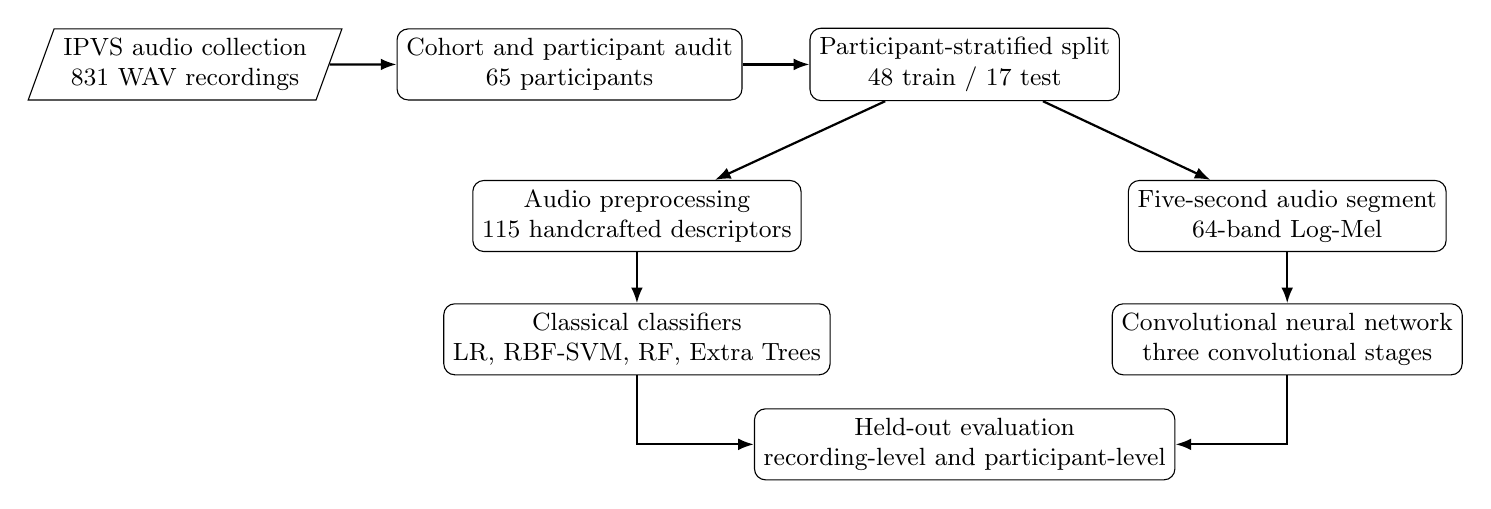
\begin{tikzpicture}[
 node distance=0.65cm and 0.85cm,
 block/.style={draw, rounded corners, align=center, minimum width=2.7cm, minimum height=0.85cm, font=\small},
 data/.style={draw, trapezium, trapezium left angle=70, trapezium right angle=110, align=center, minimum width=2.7cm, minimum height=0.85cm, font=\small},
 arr/.style={-{Latex[length=2mm]}, thick}
]
\node[data] (data) {IPVS audio collection\\831 WAV recordings};
\node[block, right=of data] (audit) {Cohort and participant audit\\65 participants};
\node[block, right=of audit] (split) {Participant-stratified split\\48 train / 17 test};
\node[block, below left=1.0cm and 0.1cm of split] (hand) {Audio preprocessing\\115 handcrafted descriptors};
\node[block, below right=1.0cm and 0.1cm of split] (mel) {Five-second audio segment\\64-band Log-Mel};
\node[block, below=of hand] (ml) {Classical classifiers\\LR, RBF-SVM, RF, Extra Trees};
\node[block, below=of mel] (cnn) {Convolutional neural network\\three convolutional stages};
\node[block, below=1.0cm of split, yshift=-2.9cm, minimum width=3.7cm] (eval) {Held-out evaluation\\recording-level and participant-level};
\draw[arr] (data)--(audit);
\draw[arr] (audit)--(split);
\draw[arr] (split)--(hand);
\draw[arr] (split)--(mel);
\draw[arr] (hand)--(ml);
\draw[arr] (mel)--(cnn);
\draw[arr] (ml.south) |- (eval.west);
\draw[arr] (cnn.south) |- (eval.east);
\end{tikzpicture}
\caption{Team-developed schematic of the two implemented audio-classification branches.}
\label{fig:pipeline}
\end{figure*}

For classical models, five-fold stratified cross-validation is conducted using training participants only. Each fold is formed at participant level, and all recordings from the fold's participants are mapped to the corresponding training or validation subset. Balanced accuracy is used to compare classifiers. This prevents participant overlap between folds, although the reported fold metric is calculated over the recordings belonging to each fold.

\subsection{Audio Preprocessing and Handcrafted Features}
Audio is loaded from WAV files and converted to mono by averaging channels when necessary. Signals are resampled to 16 kHz, mean-centred, and peak-normalised when the peak amplitude is nonzero. For a discrete recording $x[n]$, mean-centering is
\begin{equation}
x_c[n]=x[n]-\bar{x},
\end{equation}
and peak normalisation is
\begin{equation}
x_p[n]=\frac{x_c[n]}{\max_n |x_c[n]|}.
\end{equation}
The normalisation scales the maximum absolute sample; it does not remove differences in microphone, room, or speaking conditions.

The notebook extracts 20 MFCC coefficients and their delta descriptors. It additionally computes spectral centroid, spectral bandwidth, spectral rolloff, zero-crossing rate (ZCR), root-mean-square (RMS) energy, and chroma features. For each frame-based feature sequence, the mean and standard deviation are calculated. Together with the duration feature, these operations produce 115 feature columns per recording.

MFCCs summarise the short-time spectral envelope. The signal is framed and windowed, transformed using the short-time Fourier transform, mapped through Mel-spaced filters, logarithmically compressed, and decorrelated using a discrete cosine transform. Delta-MFCCs describe temporal changes in the cepstral sequence. Spectral centroid estimates the weighted centre of spectral energy; bandwidth measures its spread; rolloff identifies a frequency below which a specified proportion of energy lies; ZCR counts sign changes; RMS summarises frame energy; and chroma maps spectral energy into pitch-class bins.

For a frame-level sequence $z_1,\ldots,z_T$, the summary statistics are
\begin{equation}
\mu_z=\frac{1}{T}\sum_{t=1}^{T}z_t,\qquad
\sigma_z=\sqrt{\frac{1}{T}\sum_{t=1}^{T}(z_t-\mu_z)^2}.
\end{equation}
The fixed-length summaries permit conventional classifiers to process recordings with different durations.

\subsection{Classical Machine-Learning Models}
Four classifiers are evaluated: Logistic Regression, an RBF-kernel SVM, Random Forest, and Extra Trees. Median imputation and standardisation are included in the Logistic Regression and SVM pipelines. The tree-based pipelines use median imputation without standardisation. Class weighting is enabled. The SVM is selected because it obtains the highest mean balanced accuracy in the five training-participant folds.

\begin{table}[!t]
\centering
\caption{Five-fold participant-stratified cross-validation results}
\label{tab:cv}
\begin{tabular}{lcc}
\toprule
Classifier & Mean BA & Std. dev.\\
\midrule
RBF-SVM & 0.9606 & 0.0360\\
Extra Trees & 0.9483 & 0.0474\\
Random Forest & 0.9404 & 0.0469\\
Logistic Regression & 0.9328 & 0.0302\\
\bottomrule
\end{tabular}
\end{table}

\subsection{Log-Mel Spectrogram and CNN}
For the CNN branch, each recording is resampled to 16 kHz and represented by a five-second segment taken from the beginning of the recording. Shorter signals are zero-padded and longer signals are truncated. The Mel spectrogram uses 64 Mel bands, an FFT size of 1024, and a hop length of 256 samples. Power values are converted to decibels relative to the maximum value. Each input has shape $64\times313\times1$.

The CNN contains three convolutional stages with 16, 32, and 64 filters. The first two stages are followed by batch normalisation and max pooling. The third stage is followed by global average pooling. The classification head contains dropout (0.45), a 32-unit ReLU dense layer, dropout (0.35), and a one-unit sigmoid output. The model uses Adam with learning rate $3\times10^{-4}$ and binary cross-entropy. Training is limited to 60 epochs with batch size 16, early stopping (validation-loss patience 8), and learning-rate reduction on plateau (factor 0.5, patience 3, minimum learning rate $10^{-6}$).

The 48 development participants are split into 38 training and 10 validation participants. The 17 held-out test participants remain unchanged. Sample weights are constructed so that participants contribute equally overall, followed by participant-level class balancing.

\begin{table}[!t]
\centering
\caption{CNN configuration}
\label{tab:cnn}
\begin{tabular}{ll}
\toprule
Component & Configuration\\
\midrule
Input & $64\times313\times1$\\
Convolution filters & 16, 32, 64\\
Kernel size & $3\times3$\\
Pooling & Max pooling after stages 1 and 2\\
Aggregation & Global average pooling\\
Dense layer & 32 units, ReLU\\
Dropout & 0.45 and 0.35\\
Output & 1 unit, sigmoid\\
Optimizer & Adam, $3\times10^{-4}$\\
Loss & Binary cross-entropy\\
Batch / maximum epochs & 16 / 60\\
\bottomrule
\end{tabular}
\end{table}

\subsection{Evaluation Metrics and Participant Aggregation}
The study reports accuracy, balanced accuracy, PD precision, PD recall, F1-score, and ROC-AUC. Accuracy is the fraction of correct predictions. Balanced accuracy is the mean of sensitivity and specificity. Precision measures the proportion of positive predictions that are correct; recall measures the proportion of PD cases detected; F1 is their harmonic mean; and ROC-AUC measures ranking performance across thresholds.

For participant-level evaluation, recording-level PD probabilities are averaged within each participant. If participant $q$ has $R_q$ recordings, the aggregate score is
\begin{equation}
\bar{p}_q=\frac{1}{R_q}\sum_{r=1}^{R_q}p_{qr}.
\end{equation}
A participant is assigned to the PD class when $\bar{p}_q\geq0.5$. This is a distinct evaluation unit from an individual recording.

\section{Experimental Results}
The selected RBF-SVM is evaluated on 226 held-out recordings from 17 participants. The CNN is evaluated on the same test recordings. Table~\ref{tab:results} reports the metrics at both recording and participant levels.

\begin{table*}[!t]
\centering
\caption{Held-out test performance for the two implemented models}
\label{tab:results}
\begin{tabular}{llrrrrrr}
\toprule
Model & Evaluation unit & $n$ & Accuracy & Balanced acc. & PD precision & PD recall & PD F1 / AUC\\
\midrule
RBF-SVM & Recording & 226 & 0.9558 & 0.9568 & 0.9358 & 0.9714 & 0.9533 / 0.9939\\
CNN & Recording & 226 & 0.9690 & 0.9692 & 0.9623 & 0.9714 & 0.9668 / 0.9892\\
RBF-SVM & Participant & 17 & 0.9412 & 0.9500 & 0.8750 & 1.0000 & 0.9333 / 1.0000\\
CNN & Participant & 17 & 0.9412 & 0.9500 & 0.8750 & 1.0000 & 0.9333 / 1.0000\\
\bottomrule
\end{tabular}
\end{table*}

At recording level, the CNN has higher accuracy (0.9690 versus 0.9558), balanced accuracy (0.9692 versus 0.9568), precision, and F1-score. Both models have the same PD recall (0.9714). The SVM has a higher ROC-AUC (0.9939 versus 0.9892). Thus, the comparison does not yield a single model that dominates every metric. No statistical significance test is implemented, so these numerical differences should not be described as statistically significant.

At participant level, both models have the same reported metrics: 0.9412 accuracy, 0.9500 balanced accuracy, 0.8750 PD precision, 1.0000 PD recall, 0.9333 F1-score, and 1.0000 ROC-AUC. The participant test set contains only 17 people, so one participant corresponds to approximately 5.9 percentage points of accuracy. The 226 recordings are repeated observations from those 17 participants and must not be interpreted as 226 independent subjects.

\begin{figure*}[!t]
\centering
\includegraphics[width=0.82\textwidth]{recording_confusion_matrices.png}
\caption{Recording-level confusion matrices reconstructed from the notebook's held-out classification reports. Rows indicate true classes and columns indicate predicted classes.}
\label{fig:confusion}
\end{figure*}

\subsection{Exploratory Feature Importance}
Permutation importance is computed for the selected SVM using balanced accuracy on the held-out test recordings. The largest mean importance values in the saved output include MFCC means, chroma variability, MFCC standard deviations, delta-MFCC, spectral bandwidth, spectral rolloff, and RMS variability. Fig.~\ref{fig:importance} shows the ten highest-ranked entries in the saved output.

\begin{figure}[!t]
\centering
\includegraphics[width=\columnwidth]{permutation_importance.png}
\caption{Top ten SVM permutation-importance features from the saved notebook output.}
\label{fig:importance}
\end{figure}

Permutation importance is conditional on the fitted model, dataset, and evaluation sample. Correlated descriptors may share predictive information. The ranking is exploratory and does not establish causality, a biological mechanism, or a clinically validated biomarker.

\section{Discussion}
The participant-aware split is an important design choice because it prevents recordings from the same individual from appearing in both training and held-out testing. The separate participant-level results provide a more direct view of performance on unseen people than file-level scores alone. Nevertheless, the participant test set is small, and its metrics have limited precision.

The two approaches show complementary behaviour. The CNN is stronger on several recording-level threshold metrics, while the SVM has the higher recording-level ROC-AUC. Their participant-level scores are identical in this saved run. These observations are specific to this dataset, split, and training procedure. They do not demonstrate that CNNs or SVMs are generally preferable for PD voice classification.

The study should also be interpreted in light of the related literature. Reviews describe substantial variation in datasets, language, speech tasks, feature definitions, and validation procedures \cite{ngo2022,amato2023,xavier2025,malekroodi2025}. Consequently, direct numerical comparisons with published results are not justified unless experimental conditions are matched. The ISNDAM paper is relevant background, but its datasets, algorithm, and statistical testing differ from the present implementation \cite{luna2023}.

\section{Limitations and Future Work}
The experiment uses one dataset and one saved participant-level train/test split, with only 17 held-out participants. The healthy-control class combines young and elderly cohorts; age and cohort composition may therefore influence the acoustic patterns. Recording devices, environments, tasks, language, and speaking styles may also affect the signal. The CNN uses only the first five seconds of each recording, potentially omitting useful information later in the utterance.

The notebook does not report external-dataset validation, prospective clinical evaluation, probability calibration, or repeated independent test splits. Future work should evaluate additional participants and independent datasets, use repeated grouped or nested grouped validation, test different segment-selection strategies, assess recording-condition robustness, and examine calibration and uncertainty. Clinical application would require prospective validation and expert oversight.

\section{Conclusion}
This project implemented two participant-aware voice-classification pipelines for the IPVS collection: a classical pipeline using 115 handcrafted acoustic feature columns and a CNN using five-second Log-Mel spectrograms. The RBF-SVM achieved 0.9558 recording-level accuracy and 0.9412 participant-level accuracy. The CNN achieved 0.9690 recording-level accuracy and the same participant-level accuracy. The models therefore show promising discrimination within the saved experiment, but the small held-out participant cohort, single dataset, and single split prevent broad generalisation claims. The work is an experimental research prototype and not a clinical diagnostic system.

\section*{Author Contributions}
Suvinay Foujdar: project coordination, integration of the experimental pipeline, experimental design, and manuscript preparation. Akshat Goyal: dataset organisation, audio preprocessing, handcrafted-feature extraction, and classical machine-learning experiments. Navya Loshali: literature review, Log-Mel CNN experiments, result visualisation, and manuscript review. 

\section*{Acknowledgment}
The authors acknowledge Bennett University for the academic setting in which this project was completed. The authors acknowledge the providers of the IPVS dataset and the researchers whose work is cited. Specific funding or individual assistance should be added only if it was actually received.
\balance
\begin{thebibliography}{9}
\scriptsize
\bibitem{luna2023}
I. Luna-Ortiz, M. Aldape-Pérez, A. V. Uriarte-Arcia, A. Rodríguez-Molina, A. Alarcón-Paredes, and E. Ventura-Molina, ``Parkinson's Disease Detection from Voice Recordings Using Associative Memories,'' \emph{Healthcare}, vol. 11, no. 11, Art. no. 1601, 2023, doi: 10.3390/healthcare11111601.

\bibitem{ngo2022}
Q. C. Ngo, M. A. Motin, N. D. Pah, P. Drotár, P. Kempster, and D. Kumar, ``Computerized analysis of speech and voice for Parkinson's disease: A systematic review,'' \emph{Computer Methods and Programs in Biomedicine}, vol. 226, Art. no. 107133, 2022, doi: 10.1016/j.cmpb.2022.107133.

\bibitem{amato2023}
F. Amato, G. Saggio, V. Cesarini, G. Olmo, and G. Costantini, ``Machine learning- and statistical-based voice analysis of Parkinson's disease patients: A survey,'' \emph{Expert Systems with Applications}, vol. 219, Art. no. 119651, 2023, doi: 10.1016/j.eswa.2023.119651.

\bibitem{xavier2025}
D. Xavier, V. Felizardo, B. Ferreira, H. Zacarias, M. Pourvahab, L. Souza-Pereira, and N. M. Garcia, ``Voice analysis in Parkinson's disease---a systematic literature review,'' \emph{Artificial Intelligence in Medicine}, vol. 163, Art. no. 103109, 2025, doi: 10.1016/j.artmed.2025.103109.

\bibitem{malekroodi2025}
H. Sedigh Malekroodi, B.-I. Lee, and M. Yi, ``Voice-Based Detection of Parkinson's Disease Using Machine and Deep Learning Approaches: A Systematic Review,'' \emph{Bioengineering}, vol. 12, no. 11, Art. no. 1279, 2025, doi: 10.3390/bioengineering12111279.

\bibitem{hossain2026}
M. A. Hossain, E. Traini, and F. Amenta, ``Identification of Parkinson's Disease from Native Italian People: Machine Learning Voice Analysis,'' \emph{BioMed}, vol. 6, no. 3, Art. no. 15, 2026, doi: 10.3390/biomed6030015.
\end{thebibliography}

\end{document}
